\documentclass[border=6pt]{standalone}
\usepackage[T1]{fontenc}
\usepackage{courier}
\usepackage[scaled=0.95]{helvet}
\renewcommand{\familydefault}{\sfdefault}
\usepackage{sfmath}
\usepackage[version=4]{mhchem}
\usepackage{tikz}
\usepackage{pgfplots}
\pgfplotsset{compat=newest}
\usetikzlibrary{arrows.meta,positioning,calc,fit,backgrounds,shapes.geometric,decorations.pathreplacing,patterns}
\definecolor{ink}{HTML}{17233A}
\definecolor{inksoft}{HTML}{44506A}
\definecolor{teal}{HTML}{0E6B6B}
\definecolor{tealsoft}{HTML}{E5F0EF}
\definecolor{amber}{HTML}{B26B12}
\definecolor{ambersoft}{HTML}{FBF0DF}
\definecolor{blue}{HTML}{2F6690}
\definecolor{bluesoft}{HTML}{E3ECF4}
\definecolor{plum}{HTML}{7A4D8C}
\definecolor{plumsoft}{HTML}{EFE7F3}
\definecolor{greyc}{HTML}{8A94A3}
\definecolor{linec}{HTML}{D3DCE1}
\definecolor{oxy}{HTML}{C0392B}
\definecolor{carb}{HTML}{3B4252}
\definecolor{hyd}{HTML}{E6E9EE}
\definecolor{nit}{HTML}{2F6690}
\tikzset{
  every picture/.style={line cap=round,line join=round},
  lab/.style={font=\small, text=inksoft},
  >={Stealth[length=7pt]},
}
\pgfplotsset{
  every axis/.append style={axis line style={inksoft}, tick style={inksoft}, tick label style={font=\footnotesize, text=inksoft}, label style={font=\small, text=ink}},
}
% fragment tile: \frag{node name}{position}{colour}{content}
\newcommand{\frag}[4]{\node[draw=#3, fill=#3!12, line width=1.4pt, rounded corners=6pt, minimum width=1.25cm, minimum height=1.05cm, text=#3, font=\bfseries] (#1) at (#2) {#4};}
\newcommand{\ring}{\tikz[baseline=-0.6ex]{\draw[line width=1.1pt] (0:0.3)--(60:0.3)--(120:0.3)--(180:0.3)--(240:0.3)--(300:0.3)--cycle; \draw[line width=0.8pt] (0,0) circle (0.16);}}
\newcommand{\bond}[2]{\draw[ink, line width=2.2pt] (#1) -- (#2);}

\begin{document}
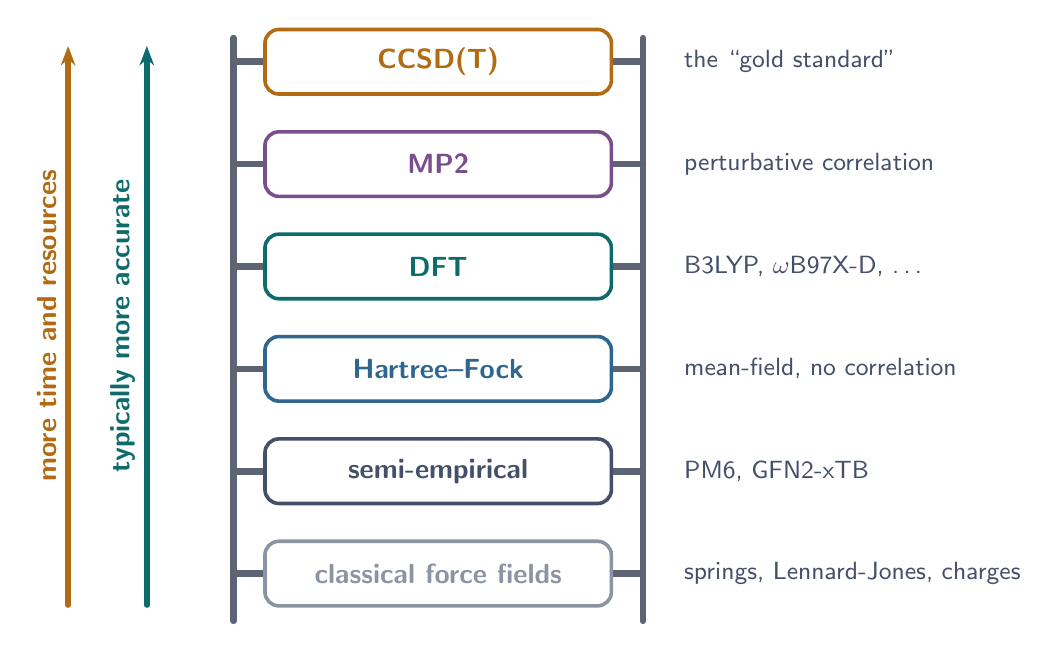
\begin{tikzpicture}
\draw[ink!70, line width=2.4pt] (0,-0.4) -- (0,7.0); \draw[ink!70, line width=2.4pt] (5.2,-0.4) -- (5.2,7.0);
\draw[ink!70, line width=2.4pt] (0,0.20) -- (5.2,0.20);
\node[fill=white, draw=greyc, line width=1.3pt, rounded corners=5pt, minimum width=4.4cm, minimum height=0.82cm, font=\bfseries, text=greyc] (r0) at (2.6,0.20) {classical force fields};
\node[font=\small, text=inksoft, anchor=west] at (5.6,0.20) {springs, Lennard-Jones, charges};
\draw[ink!70, line width=2.4pt] (0,1.50) -- (5.2,1.50);
\node[fill=white, draw=inksoft, line width=1.3pt, rounded corners=5pt, minimum width=4.4cm, minimum height=0.82cm, font=\bfseries, text=inksoft] (r1) at (2.6,1.50) {semi-empirical};
\node[font=\small, text=inksoft, anchor=west] at (5.6,1.50) {PM6, GFN2-xTB};
\draw[ink!70, line width=2.4pt] (0,2.80) -- (5.2,2.80);
\node[fill=white, draw=blue, line width=1.3pt, rounded corners=5pt, minimum width=4.4cm, minimum height=0.82cm, font=\bfseries, text=blue] (r2) at (2.6,2.80) {Hartree--Fock};
\node[font=\small, text=inksoft, anchor=west] at (5.6,2.80) {mean-field, no correlation};
\draw[ink!70, line width=2.4pt] (0,4.10) -- (5.2,4.10);
\node[fill=white, draw=teal, line width=1.3pt, rounded corners=5pt, minimum width=4.4cm, minimum height=0.82cm, font=\bfseries, text=teal] (r3) at (2.6,4.10) {DFT};
\node[font=\small, text=inksoft, anchor=west] at (5.6,4.10) {B3LYP, \(\omega\)B97X-D, \dots};
\draw[ink!70, line width=2.4pt] (0,5.40) -- (5.2,5.40);
\node[fill=white, draw=plum, line width=1.3pt, rounded corners=5pt, minimum width=4.4cm, minimum height=0.82cm, font=\bfseries, text=plum] (r4) at (2.6,5.40) {MP2};
\node[font=\small, text=inksoft, anchor=west] at (5.6,5.40) {perturbative correlation};
\draw[ink!70, line width=2.4pt] (0,6.70) -- (5.2,6.70);
\node[fill=white, draw=amber, line width=1.3pt, rounded corners=5pt, minimum width=4.4cm, minimum height=0.82cm, font=\bfseries, text=amber] (r5) at (2.6,6.70) {CCSD(T)};
\node[font=\small, text=inksoft, anchor=west] at (5.6,6.70) {the ``gold standard''};
\draw[teal, line width=2pt, ->] (-1.1,-0.2) -- (-1.1,6.9) node[midway, rotate=90, above, font=\bfseries, text=teal] {typically more accurate};
\draw[amber, line width=2pt, ->] (-2.1,-0.2) -- (-2.1,6.9) node[midway, rotate=90, above, font=\bfseries, text=amber] {more time and resources};
% To mark the GMD reference level, uncomment and set the rung (r0 ... r5):
% \node[fill=teal, text=white, font=\small\bfseries, rounded corners=3pt, anchor=east] at ($(r3.west)+(-0.15,0)$) {GMD data};
\end{tikzpicture}
\end{document}
